\documentclass{article}

% if you need to pass options to natbib, use, e.g.:
%     \PassOptionsToPackage{numbers, compress}{natbib}
% before loading neurips_2018

% ready for submission
% \usepackage{neurips_2018}

% to compile a preprint version, e.g., for submission to arXiv, add add the
% [preprint] option:
    \usepackage[preprint]{neurips_2018}

% to compile a camera-ready version, add the [final] option, e.g.:
 %    \usepackage[final]{neurips_2018}

% to avoid loading the natbib package, add option nonatbib:
%     \usepackage[nonatbib]{neurips_2018}

\usepackage[utf8]{inputenc} % allow utf-8 input
\usepackage[T1]{fontenc}    % use 8-bit T1 fonts
\usepackage{hyperref}       % hyperlinks
\usepackage{url}            % simple URL typesetting
\usepackage{booktabs}       % professional-quality tables
\usepackage{amsfonts}       % blackboard math symbols
\usepackage{nicefrac}       % compact symbols for 1/2, etc.
\usepackage{microtype}      % microtypography
%\usepackage{amsthm}
\usepackage{amssymb}
\usepackage{mathtools}
\DeclarePairedDelimiter\abs{\lvert}{\rvert}
\DeclarePairedDelimiter\norm{\lVert}{\rVert}
\DeclarePairedDelimiter\inner{\langle}{\rangle}
\def\P{\mathcal{P}}
\DeclarePairedDelimiter\floor{\lfloor}{\rfloor}
\DeclarePairedDelimiter\ceil{\lceil}{\rceil}

\DeclareMathOperator*{\argmin}{argmin}

\usepackage{algorithm}
\usepackage{algorithmic}
\makeatletter
\newcommand{\algorithmicfunction}{\textbf{function}}
\newcommand{\algorithmicendfunction}{\algorithmicend\ \algorithmicfunction}
\newenvironment{ALC@func}{\begin{ALC@g}}{\end{ALC@g}}
\newcommand{\FUNCTION}[2][default]{\ALC@it\algorithmicfunction\ #2\ %
\textbf{:}%
\ALC@com{#1}\begin{ALC@func}}
\ifthenelse{\boolean{ALC@noend}}{
    \newcommand{\ENDFUNCTION}{\end{ALC@func}}
  }{
    \newcommand{\ENDFUNCTION}{\end{ALC@func}\ALC@it\algorithmicendfunction}
  }
\makeatother

\title{A practical information theoretic clustering method}

% The \author macro works with any number of authors. There are two commands
% used to separate the names and addresses of multiple authors: \And and \AND.
%
% Using \And between authors leaves it to LaTeX to determine where to break the
% lines. Using \AND forces a line break at that point. So, if LaTeX puts 3 of 4
% authors names on the first line, and the last on the second line, try using
% \AND instead of \And before the third author name.

\author{%
  David S.~Hippocampus\thanks{Use footnote for providing further information
    about author (webpage, alternative address)---\emph{not} for acknowledging
    funding agencies.} \\
  Department of Computer Science\\
  Cranberry-Lemon University\\
  Pittsburgh, PA 15213 \\
  \texttt{hippo@cs.cranberry-lemon.edu} \\
  % examples of more authors
  % \And
  % Coauthor \\
  % Affiliation \\
  % Address \\
  % \texttt{email} \\
  % \AND
  % Coauthor \\
  % Affiliation \\
  % Address \\
  % \texttt{email} \\
  % \And
  % Coauthor \\
  % Affiliation \\
  % Address \\
  % \texttt{email} \\
  % \And
  % Coauthor \\
  % Affiliation \\
  % Address \\
  % \texttt{email} \\
}

\begin{document}
% \nipsfinalcopy is no longer used

\maketitle

\begin{abstract}
  We propose a new hierachical clustering method based on a multivariate information metric, which is computable in polynomial time. The proposed method generate different hierachical tree by scaling the metric used. The hierachical tree can be computed efficiently in polynomial time by invoking parametric maximal flow algorithm. Experiment shows that clustering result is comparable with other hierachical clustering technique or genral clustering method.
\end{abstract}

\section{Introduction}
In traditional agglomerative clustering method, two clusters are agglomerated based on pairwise inter-cluster similarity.  For example, well-known single-linkage clustering method uses nearest distance metric between two clusters and merge the two with minimal distance\cite{RN16}.  However, pairwise comparision is not optimal since it loses information shared between more than two clusters.  To overcome this problem, we define a multivariate similarity measure starting from arbitrary pairwise similarity metrics. Using this multivariate measure in the agglomerative clustering case, we merge several clusters in one step with largest similarity and build our hierachical tree.

The multivariate measure we proposed is equivalent to graph strength \cite{RN12}, it measures the coherrent similarity shared by each component. However, this measure is compute expensive in its definitional form and cannot be used directly to merge clusters. A similar hierachical clustering method called \textbf{minimum average cost} exploits the structural property of the average cost and converts the problem to submodular function minimization\cite{RN7}. In this paper, we show that the same mathematical technique can be used and the special form of submodular function minimization is equivalent to principal sequence of partition\cite{RN3}, which can be solved efficiently by parametric maximal flow algorithm\cite{RN4}. 

The clustering method used in this paper is information theoretic since it is established on the mathematical theory of \textbf{info-clustering}\cite{RN1}. This theory mainly deals with random variable clustering and we generalize and realize it to data clustering scenario, which is the main contribution of this paper. Experiment on synthesized and real-world dataset shows the info-clustering method performs well. 

The paper is organized as follows. In Section \ref{sec:models}, we formulate the info-clustering problem and show its connection with theory. In Section \ref{sec:algorithm}, we propose the algorithm workflow to solve the info-clustering problem. In Section \ref{sec:experiment}, we give the experiement result and comparision of info-clustering with other methods. Finally, we give the conclusion in Section \ref{sec:conclusion}.


\section{Models}\label{sec:models}

Consider an undirected graph partition problem, in which we want to partition the graph nodes into several groups with largest similarity within each group and smallest similarity between different group. To formulate this problem mathematically, the graph is denoted by $G(V,E)$, with vertex set $V = \{1, 2, \dots, \abs{V}\}$ and edge set $E=\{(i,j) | w_{ij}>0\}$ where the edge weight $w$ is nonnegative and represents pairwise similarity of nodes. We use $\Pi'$ to denote the collection of non-trival paritions of graph $G$. The clustering criterion is to minimize the following quantity over different parition of $V$
\begin{definition}[Multivariate similarity]\label{def:ms}
\begin{align}
I_{\P}(Z_V) & = {1 \over 2 ( \abs{\mathcal{P}} - 1) } \sum_{\substack{i\in C, j \not\in C\\ C\in \mathcal{P}}} w_{ij} \\
I(Z_V) & = \min_{\mathcal{P} \in \Pi'(V)} I_{\mathcal{P}}(Z_V)  \label{eq:ms}
\end{align}
\end{definition}

We call the quantity in equation \eqref{eq:ms} \textbf{multivariate similarity} because it measures the similarity shared by multiple graph nodes. The definition has the same form with that of graph strength if  the whole graph nodes are considered\cite{RN12}. However, we can compute multivariate similarity for any subset of $V$. In such case, 
we use subgraph symbol $V'$ to replace $V$ in equation \eqref{eq:ms}.

For example, for a three node graph $G=(\{1,2,3\},\{(1,2),(1,3),(2,3)| w_{12}=w_{23}=1, w_{13}=5\})$, we have $I(Z_{\{1,3\}}) = 5$ and $I(Z_V) = 2$ which is minimal value among $I_{\{1\},\{2\},\{3\}}(Z_V)=3.5, I_{\{1, 2\},\{3\}}(Z_V)=6, I_{\{1,3\},\{2\}}(Z_V)=2, I_{\{1\},\{2,3\}}(Z_V)=6$.


Based on the definition \eqref{def:ms}, we have both a top-down and bottom-up version of hierachical clustering.
\begin{proposition}\label{prop:ta}
The following two procedures generate the same hierachical tree, illustrated by figure \ref{fig:ta}.
\begin{enumerate}
\item For a graph $G$, suppose $I_{\P}(Z_V)=I(Z_V)$, each subset of $\P$ is child of hierachical tree root $V$. For each tree leaf node, use \eqref{eq:ms} to split it until the leaf node has exactly one element.
\item For a graph $G$, suppose $I(Z_C) = \max_{B\subseteq V} I(Z_B)$ and $C$ is maximal, merge singleton element of $C$ together and $G$ is contracted. At each step select the set with maximal multivariate similarity to contract the graph until the graph contracted to one vertex.
\end{enumerate}
\end{proposition}
%proof in attachment.
For the top-down approach, there may be multiple partition $\P$ that reaches the minimum in \eqref{eq:ms}, we can show that there is a unique finest partition and this one is used; for the bottom-up approach, there may be multiple subsets with equal maximal multivariate similarity, we can show that the union of these subsets also reach the maximal and maximal $C$ is unique.
%proof in attachment. (2 statements)
\begin{figure}
\centering
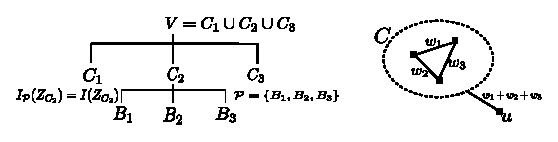
\includegraphics[width=0.8\textwidth]{two_approach.eps}
\caption{hierachical tree generation based on multivariate similarity. Left figure shows the top-down approach with each subset splitted. Right figure shows the bottom-up approach with the graph contracted.}\label{fig:ta}
\end{figure}

Using $I(Z_V)$ to cluster data directly is computing expensive, the same clustering result can be achieved by solving the following optimalization problem for all $\lambda$
\begin{proposition}
\begin{equation}\label{eq:hL}
h(\lambda) = \min_{\P \in \Pi'(V)}\{ \sum_{\substack{i\in C, j \not\in C\\ C\in \mathcal{P}}}w_{ij} - \abs{\P} \lambda \}
\end{equation}
\end{proposition}
%proof in attachment

For given $\P$, the function about $\lambda$ is linear, therefore $h(\lambda)$ is piecewise linear and we can use the parametric maximal flow algorithm to compute efficiently, which is shown in the next section.

The method is information theoretic since it is an extension of mutual information in information theory. When the graph node is random variable and the edge weight is mutual information metric, then equation \eqref{eq:ms} becomes one form of multivariate mutual information proposed in \cite{RN1}. When $I(Z_V)=0$, the random variables $Z_i$ are pairwise independent. 

\section{Algorithm}\label{sec:algorithm}

In this section, we review the basic theory to solve equation \eqref{eq:hL} and give the detailed pseudocode based on the work of \cite{RN4}.

We use $f(C)$ to denote the function defined on subsets of graph vertex set. The function is defined as
\begin{equation}
f(C) = \frac{1}{2} \sum_{ i\in C, j\in V\backslash C} w_{ij}
\end{equation}
Then we call $h(\lambda)$ the Dilworth truncation of function $f(C)$ and the computation of $h(\lambda)$ can be done by the algorithmic pyramid shown in figure \ref{fig:pyramid}. The method, called graph principal sequence of paritition and is divided into three level.
\begin{figure}
\centering
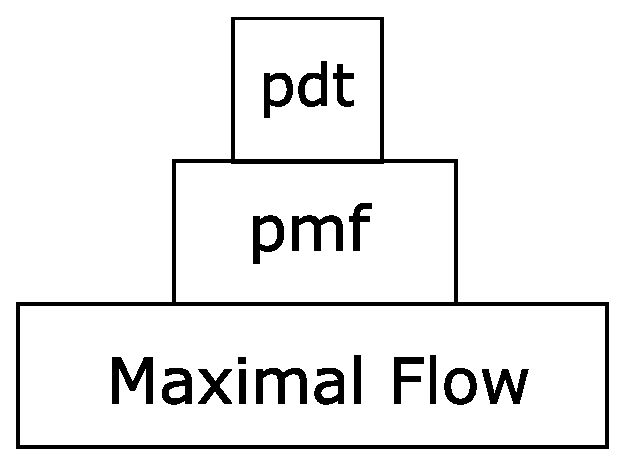
\includegraphics[width=6cm]{pdt.eps}
\caption{Algorithmic pyramid of principal sequence of partition. The top level is parametric Dilworth truncation; the middle level is parametric maximal flow and the bottom level is maximal flow}\label{fig:pyramid}
\end{figure}

\subsection{Headings: second level}

Second-level headings should be in 10-point type.

\subsubsection{Headings: third level}

Third-level headings should be in 10-point type.

\paragraph{Paragraphs}

There is also a \verb+\paragraph+ command available, which sets the heading in
bold, flush left, and inline with the text, with the heading followed by 1\,em
of space.

\section{Experiement}\label{sec:experiment}

These instructions apply to everyone.

\subsection{Citations within the text}

The \verb+natbib+ package will be loaded for you by default.  Citations may be
author/year or numeric, as long as you maintain internal consistency.  As to the
format of the references themselves, any style is acceptable as long as it is
used consistently.

The documentation for \verb+natbib+ may be found at
\begin{center}
  \url{http://mirrors.ctan.org/macros/latex/contrib/natbib/natnotes.pdf}
\end{center}
Of note is the command \verb+\citet+, which produces citations appropriate for
use in inline text.  For example,
\begin{verbatim}
   \citet{hasselmo} investigated\dots
\end{verbatim}
produces
\begin{quote}
  Hasselmo, et al.\ (1995) investigated\dots
\end{quote}

If you wish to load the \verb+natbib+ package with options, you may add the
following before loading the \verb+neurips_2018+ package:
\begin{verbatim}
   \PassOptionsToPackage{options}{natbib}
\end{verbatim}

If \verb+natbib+ clashes with another package you load, you can add the optional
argument \verb+nonatbib+ when loading the style file:
\begin{verbatim}
   \usepackage[nonatbib]{neurips_2018}
\end{verbatim}

As submission is double blind, refer to your own published work in the third
person. That is, use ``In the previous work of Jones et al.\ [4],'' not ``In our
previous work [4].'' If you cite your other papers that are not widely available
(e.g., a journal paper under review), use anonymous author names in the
citation, e.g., an author of the form ``A.\ Anonymous.''

\subsection{Footnotes}

Footnotes should be used sparingly.  If you do require a footnote, indicate
footnotes with a number\footnote{Sample of the first footnote.} in the
text. Place the footnotes at the bottom of the page on which they appear.
Precede the footnote with a horizontal rule of 2~inches (12~picas).

Note that footnotes are properly typeset \emph{after} punctuation
marks.\footnote{As in this example.}

\subsection{Figures}

\begin{figure}
  \centering
  \fbox{\rule[-.5cm]{0cm}{4cm} \rule[-.5cm]{4cm}{0cm}}
  \caption{Sample figure caption.}
\end{figure}

All artwork must be neat, clean, and legible. Lines should be dark enough for
purposes of reproduction. The figure number and caption always appear after the
figure. Place one line space before the figure caption and one line space after
the figure. The figure caption should be lower case (except for first word and
proper nouns); figures are numbered consecutively.

You may use color figures.  However, it is best for the figure captions and the
paper body to be legible if the paper is printed in either black/white or in
color.

\subsection{Tables}

All tables must be centered, neat, clean and legible.  The table number and
title always appear before the table.  See Table~\ref{sample-table}.

Place one line space before the table title, one line space after the
table title, and one line space after the table. The table title must
be lower case (except for first word and proper nouns); tables are
numbered consecutively.

Note that publication-quality tables \emph{do not contain vertical rules.} We
strongly suggest the use of the \verb+booktabs+ package, which allows for
typesetting high-quality, professional tables:
\begin{center}
  \url{https://www.ctan.org/pkg/booktabs}
\end{center}
This package was used to typeset Table~\ref{sample-table}.

\begin{table}
  \caption{Sample table title}
  \label{sample-table}
  \centering
  \begin{tabular}{lll}
    \toprule
    \multicolumn{2}{c}{Part}                   \\
    \cmidrule(r){1-2}
    Name     & Description     & Size ($\mu$m) \\
    \midrule
    Dendrite & Input terminal  & $\sim$100     \\
    Axon     & Output terminal & $\sim$10      \\
    Soma     & Cell body       & up to $10^6$  \\
    \bottomrule
  \end{tabular}
\end{table}

\section{Conclusion}\label{sec:conclusion}

Do not change any aspects of the formatting parameters in the style files.  In
particular, do not modify the width or length of the rectangle the text should
fit into, and do not change font sizes (except perhaps in the
\textbf{References} section; see below). Please note that pages should be
numbered.

\section{Preparing PDF files}

Please prepare submission files with paper size ``US Letter,'' and not, for
example, ``A4.''

Fonts were the main cause of problems in the past years. Your PDF file must only
contain Type 1 or Embedded TrueType fonts. Here are a few instructions to
achieve this.

\begin{itemize}

\item You should directly generate PDF files using \verb+pdflatex+.

\item You can check which fonts a PDF files uses.  In Acrobat Reader, select the
  menu Files$>$Document Properties$>$Fonts and select Show All Fonts. You can
  also use the program \verb+pdffonts+ which comes with \verb+xpdf+ and is
  available out-of-the-box on most Linux machines.

\item The IEEE has recommendations for generating PDF files whose fonts are also
  acceptable for NeurIPS. Please see
  \url{http://www.emfield.org/icuwb2010/downloads/IEEE-PDF-SpecV32.pdf}

\item \verb+xfig+ "patterned" shapes are implemented with bitmap fonts.  Use
  "solid" shapes instead.

\item The \verb+\bbold+ package almost always uses bitmap fonts.  You should use
  the equivalent AMS Fonts:
\begin{verbatim}
   \usepackage{amsfonts}
\end{verbatim}
followed by, e.g., \verb+\mathbb{R}+, \verb+\mathbb{N}+, or \verb+\mathbb{C}+
for $\mathbb{R}$, $\mathbb{N}$ or $\mathbb{C}$.  You can also use the following
workaround for reals, natural and complex:
\begin{verbatim}
   \newcommand{\RR}{I\!\!R} %real numbers
   \newcommand{\Nat}{I\!\!N} %natural numbers
   \newcommand{\CC}{I\!\!\!\!C} %complex numbers
\end{verbatim}
Note that \verb+amsfonts+ is automatically loaded by the \verb+amssymb+ package.

\end{itemize}

If your file contains type 3 fonts or non embedded TrueType fonts, we will ask
you to fix it.

\subsection{Margins in \LaTeX{}}

Most of the margin problems come from figures positioned by hand using
\verb+\special+ or other commands. We suggest using the command
\verb+\includegraphics+ from the \verb+graphicx+ package. Always specify the
figure width as a multiple of the line width as in the example below:
\begin{verbatim}
   \usepackage[pdftex]{graphicx} ...
   \includegraphics[width=0.8\linewidth]{myfile.pdf}
\end{verbatim}
See Section 4.4 in the graphics bundle documentation
(\url{http://mirrors.ctan.org/macros/latex/required/graphics/grfguide.pdf})

A number of width problems arise when \LaTeX{} cannot properly hyphenate a
line. Please give LaTeX hyphenation hints using the \verb+\-+ command when
necessary.

\subsubsection*{Acknowledgments}

Use unnumbered third level headings for the acknowledgments. All acknowledgments
go at the end of the paper. Do not include acknowledgments in the anonymized
submission, only in the final paper.


\bibliographystyle{plain}
\bibliography{exportlist}


\end{document}
